\subsubsection*{Análise de Complexidade e Teste de Mesa - Insertion Sort}

\qquad A análise do \textit{Insertion Sort} é iniciada por meio de um teste de mesa, permitindo a visualização da execução do algoritmo passo a passo. Na sequência, apresenta-se a fundamentação matemática para os cenários de melhor, pior e médio caso.

\vspace{0.5cm}
\noindent\textbf{Teste de Mesa}

\qquad A Figura \ref{fig:insertion_mesa} demonstra a execução do \textit{Insertion Sort} em um vetor reduzido e desordenado. O procedimento acompanha a evolução das variáveis de controle, o estado do vetor a cada iteração e as comparações realizadas, ilustrando o deslocamento dos elementos à direita para a correta inserção da chave em sua posição ordenada.

\begin{figure}[htbp]
    \centering
    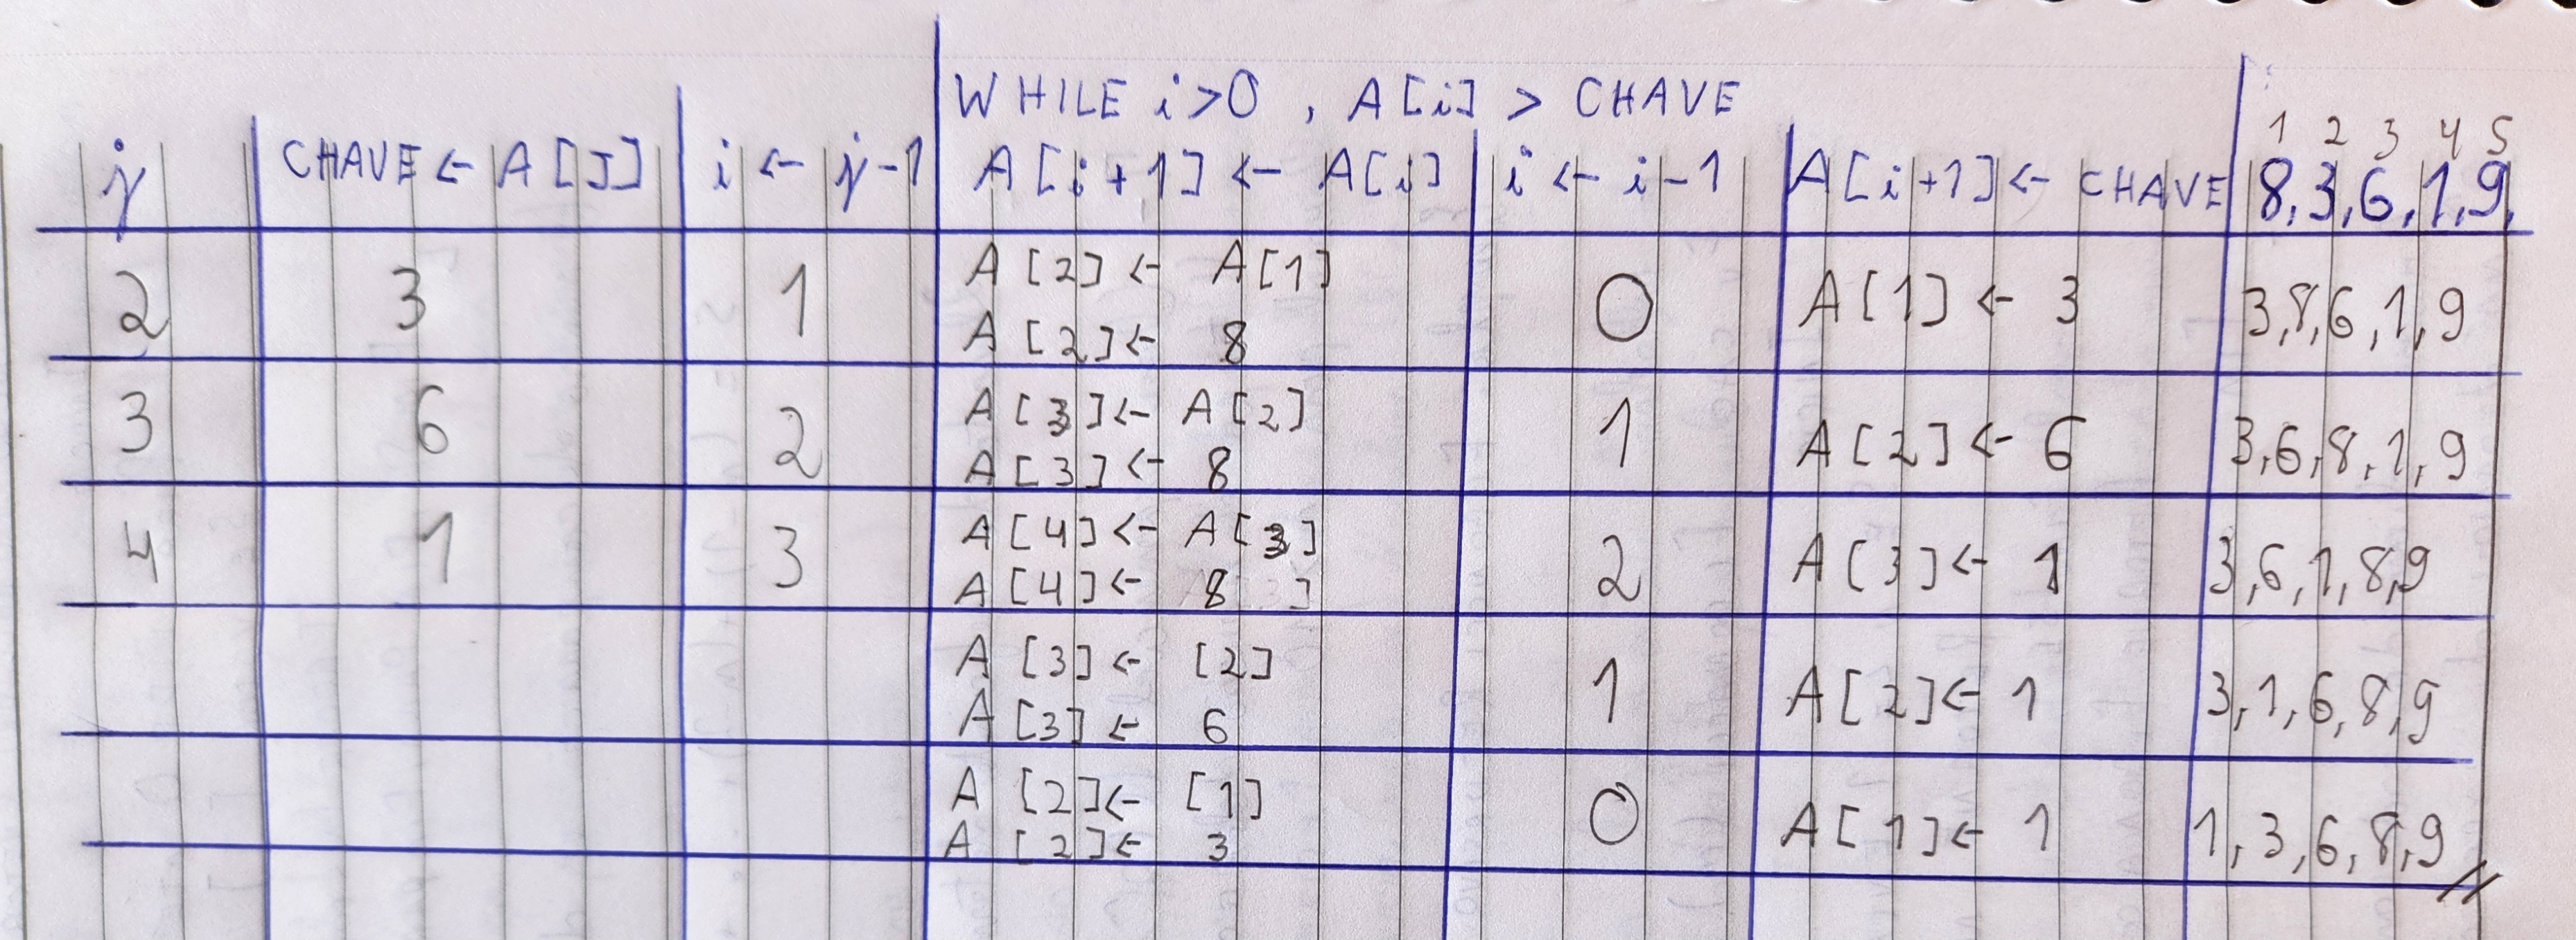
\includegraphics[width=0.9\textwidth]{Imagens/Insertion Sort/teste de mesa.jpeg}
    \caption{Teste de Mesa do algoritmo Insertion Sort (elaborado pelo autor).}
    \label{fig:insertion_mesa}
\end{figure}

\vspace{0.5cm}
\noindent\textbf{Análise Matemática de Complexidade}

\qquad A avaliação de complexidade, fundamentada na literatura clássica da área \cite{cormen}, baseia-se na tabela de custos e frequências apresentada na seção anterior. O desenvolvimento algébrico demonstrado nas Figuras \ref{fig:melhor_caso_math}, \ref{fig:pior_caso_math} e \ref{fig:medio_caso_math} elucida as variações de desempenho do algoritmo conforme a disposição inicial dos dados.

\qquad No \textbf{melhor caso} (Figura \ref{fig:melhor_caso_math}), o vetor de entrada já se encontra ordenado de forma crescente. Consequentemente, a condição do laço de repetição \texttt{while} nunca é satisfeita. O algoritmo realiza apenas uma iteração externa por elemento para verificação, ausentando-se de trocas. Esse comportamento resulta em um tempo de execução de crescimento linear, denotado por $O(n)$.

\begin{figure}[htbp]
    \centering
    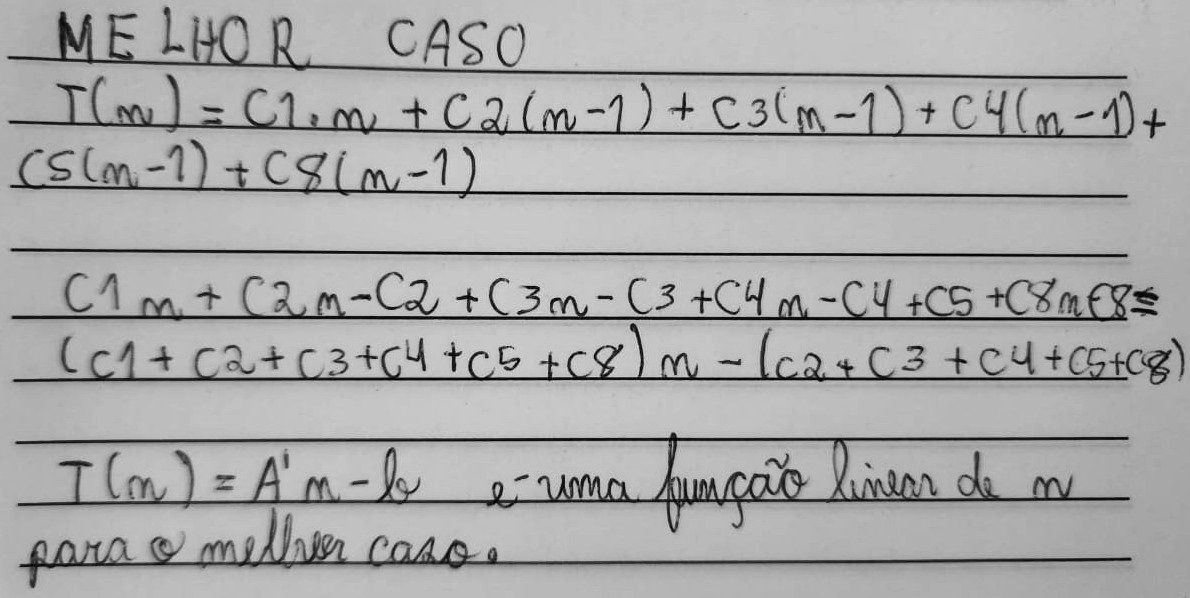
\includegraphics[width=0.6\textwidth]{Imagens/Insertion Sort/melhor caso.jpg}
    \caption{Desenvolvimento matemático da função de tempo para o Melhor Caso (elaborado pelo autor).}
    \label{fig:melhor_caso_math}
\end{figure}

\qquad O \textbf{pior caso} (Figura \ref{fig:pior_caso_math}) representa o cenário diametralmente oposto, em que o vetor está em ordem decrescente. Para cada nova chave avaliada, o algoritmo realiza o número máximo de comparações com a porção já ordenada, exigindo o deslocamento de todos os elementos precedentes. Tal comportamento gera uma quantidade massiva de operações, caracterizando um tempo de execução de crescimento quadrático ($O(n^2)$), o que o torna ineficiente para entradas extensas.

\begin{figure}[htbp]
    \centering
    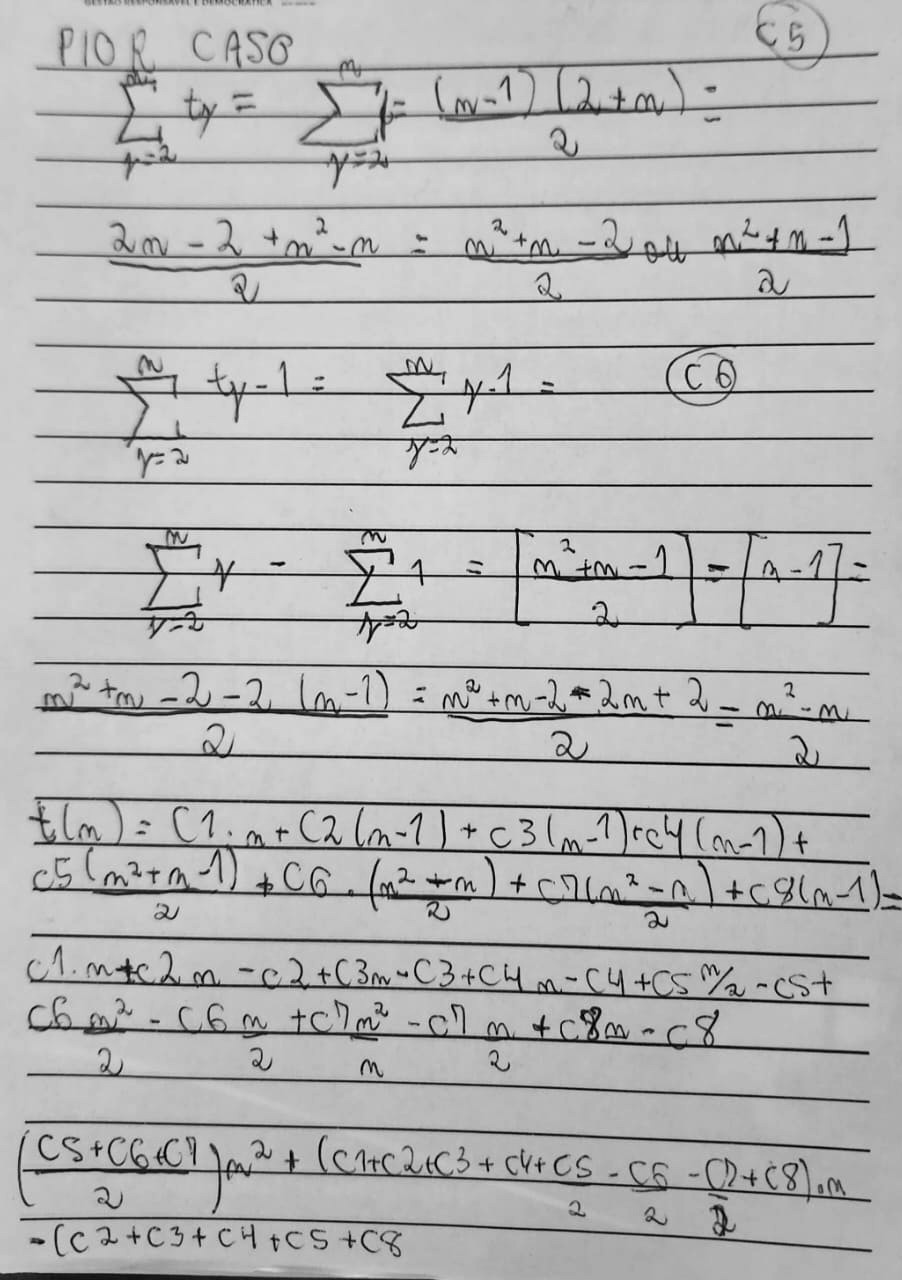
\includegraphics[width=0.7\textwidth]{Imagens/Insertion Sort/pior caso.jpg}
    \caption{Desenvolvimento matemático da função de tempo para o Pior Caso (elaborado pelo autor).}
    \label{fig:pior_caso_math}
\end{figure}

\qquad O \textbf{caso médio} (Figura \ref{fig:medio_caso_math}) ocorre quando os dados estão distribuídos de maneira aleatória. Em termos probabilísticos, o algoritmo necessita percorrer e deslocar, em média, metade dos elementos do subvetor ordenado para encontrar a posição correta de inserção. Embora o número absoluto de operações seja inferior ao do pior caso, o comportamento assintótico da função de tempo mantém o crescimento quadrático ($O(n^2)$).

\begin{figure}[htbp]
    \centering
    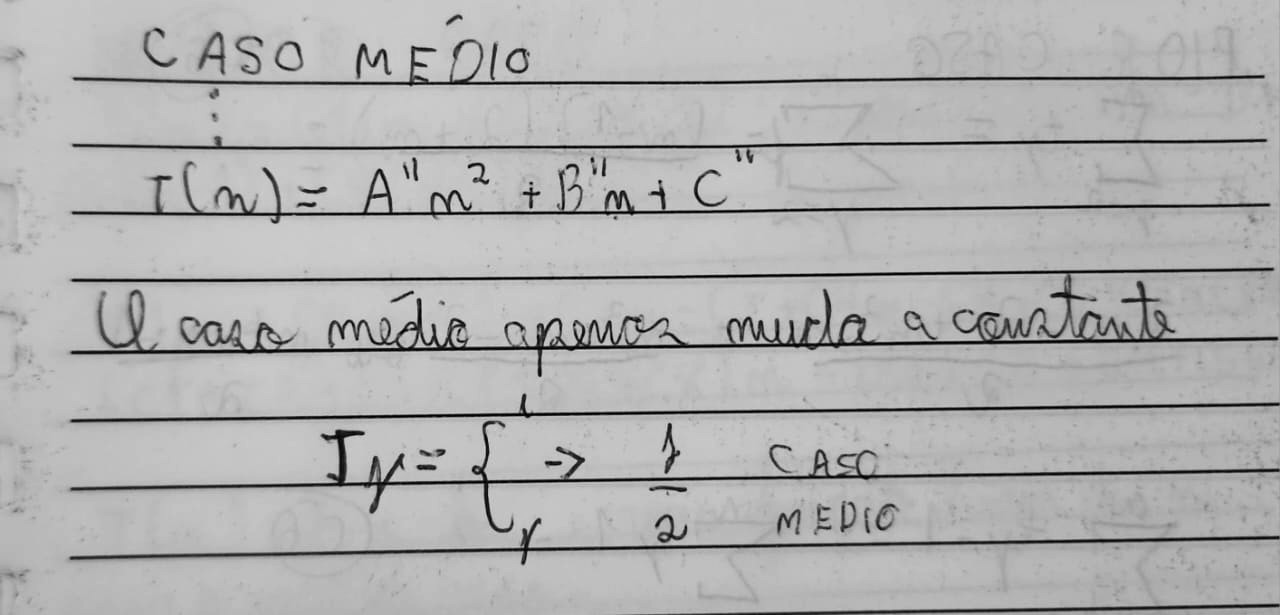
\includegraphics[width=0.8\textwidth]{Imagens/Insertion Sort/caso medio.jpg}
    \caption{Análise da função de tempo para o Caso Médio (elaborado pelo autor).}
    \label{fig:medio_caso_math}
\end{figure}

\qquad Por fim, destaca-se a eficiência espacial do \textit{Insertion Sort}. A quantidade de memória adicional requerida independe do tamanho da entrada, resultando em uma complexidade de espaço $O(1)$. Essa característica é garantida pela ordenação direta no próprio vetor original, configurando uma operação \textit{in-place}.